\documentclass[../../main.tex]{subfiles}

\begin{document}

Every robot needs a drivetrain.

\section{H-Drive}

A H-Drive consists of 4 Omni-Wheels Parallel to each other layed out in the
format of a tank drive. Then in the middle there is a aditional Omni-Wheel
perpendicular to the others.\par

Because of this an H-Drive is holonomic (can move in any direction) because when
the robot goes forward, the 4 main wheels are powered and the rollers on the secondary
wheel can slide to allow the robot to roll forward. \par

Similarly to move sidewast the secondary wheel gets powered. At the same time the rollers on
the main wheels roll to allow the robot to move. By combining the forward movement and sideways
movement, the H-Drive can move in any direction.

\begin{figure}[h]
	\centering
	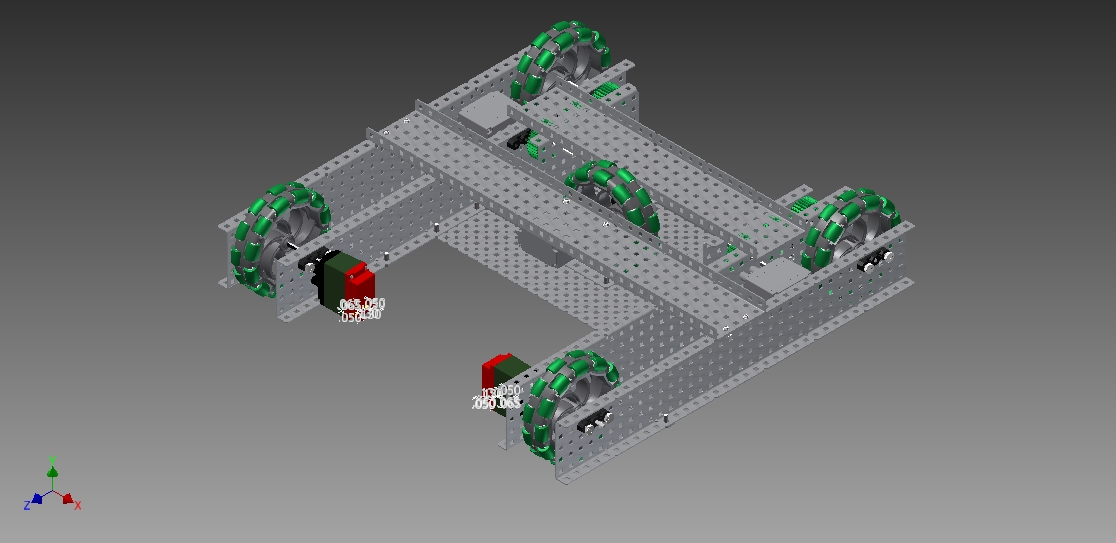
\includegraphics[height=265pt,width=\linewidth,keepaspectratio]{drivetrains/h}
	\caption{A Typical H-Drive}
	\label{fig:drivetrainh}
\end{figure}

\subsection{Advantages}

\begin{itemize}
	\item Holonomic (can move any direction)
\end{itemize}


\subsection{Disadvantages}

\begin{itemize}
	\item Easy to push sideways as only one wheel is providing
	      traction in that direction.
\end{itemize}


\section{Mecanum Drive}

<+descirption of drivetrain+>

\begin{figure}[h]
	\centering
	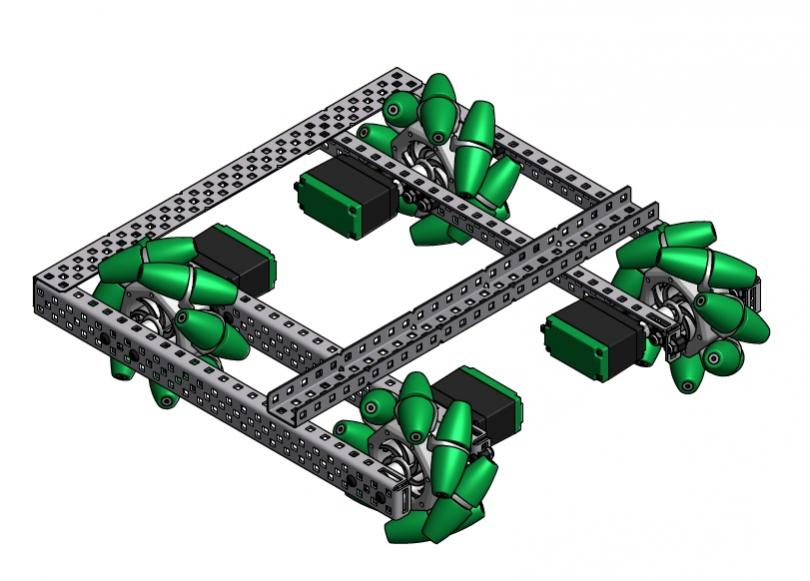
\includegraphics[height=265pt,width=\linewidth,keepaspectratio]{drivetrains/mecanum}
	\caption{A typical mecanum drive}
	\label{fig:drivetrainMecanum}
\end{figure}

\subsection{Advantages}

\begin{itemize}
	\item Holonomic
	\item Is a sqare base with 4 wheels so it can be easily converted
	      into a tank drive.
\end{itemize}


\subsection{Disadvantages}

\begin{itemize}
	\item Only moves at $\frac{1}{\sqrt{2}}$ the speed of the wheels when moving sidewast
	      negating alot of the benefit of having a holonomic drive.
	\item Requires four motors, which is half the availible motors for the v5 platform
	\item Is unstable and generaly bad at climbing over objects (we learnt this the hard
	      way in ITZ), so it will be unable to contend the center platform.
\end{itemize}



\section{Tank Drive (All Omni-Wheel)}

This style of tank drive consists of 4 Omni-Wheels in parallel to each other

\begin{figure}[h]
	\centering
	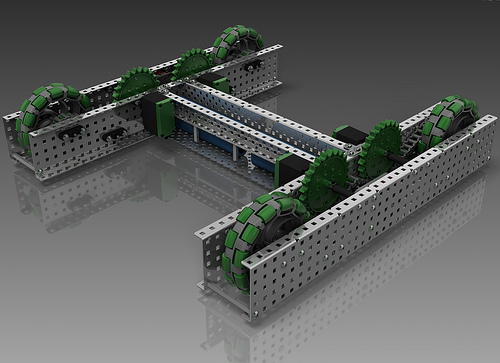
\includegraphics[height=265pt,width=\linewidth,keepaspectratio]{drivetrains/tankAllOmni}
	\caption{A typical tank drive with all omni-wheels}
	\label{fig:drivetrainTankAllOmni}
\end{figure}

\subsection{Advantages}

\begin{itemize}
	\item Has no skiding problem unlike a tank drive with all traction wheels
	\item Has the turning point in the center of the drivetrain
	\item Can easily be converted into other kinds of tank drives
\end{itemize}


\subsection{Disadvantages}

\begin{itemize}
	\item No resistanse in the sideways axis means that the robot will easily be
	      pushed off the center platform
\end{itemize}


\section{Tank Drive (All Traction Wheels)}

This drivetrain consists of 4 Tracion wheels parallel to each other

\begin{figure}[h]
	\centering
	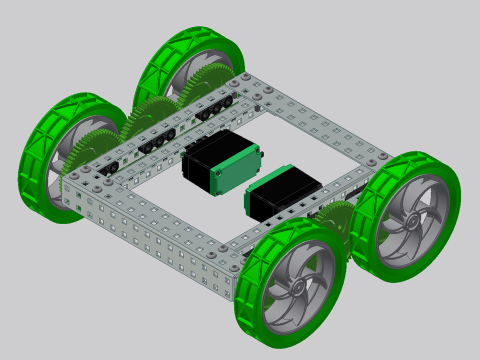
\includegraphics[height=265pt,width=\linewidth,keepaspectratio]{drivetrains/tankAllTraction}
	\caption{A typical tank drive with all traction wheels}
	\label{fig:drivetrainTankAllTraction}
\end{figure}

\subsection{Advantages}

\begin{itemize}
	\item Very strong and stable so will be better at staying on the center platform
	\item Can easily be converted into other kinds of tank drives
\end{itemize}


\subsection{Disadvantages}

\begin{itemize}
	\item Will skid when turning, causing unpredictable autonamuses and impercision for the driver
\end{itemize}


\section{Tank Drive (Half Omni, Half Tracion)}

This variant of a tank drive consists of a pair of tank wheels on one end
and a pair of omni-wheels on the other

\begin{figure}[h]
	\centering
	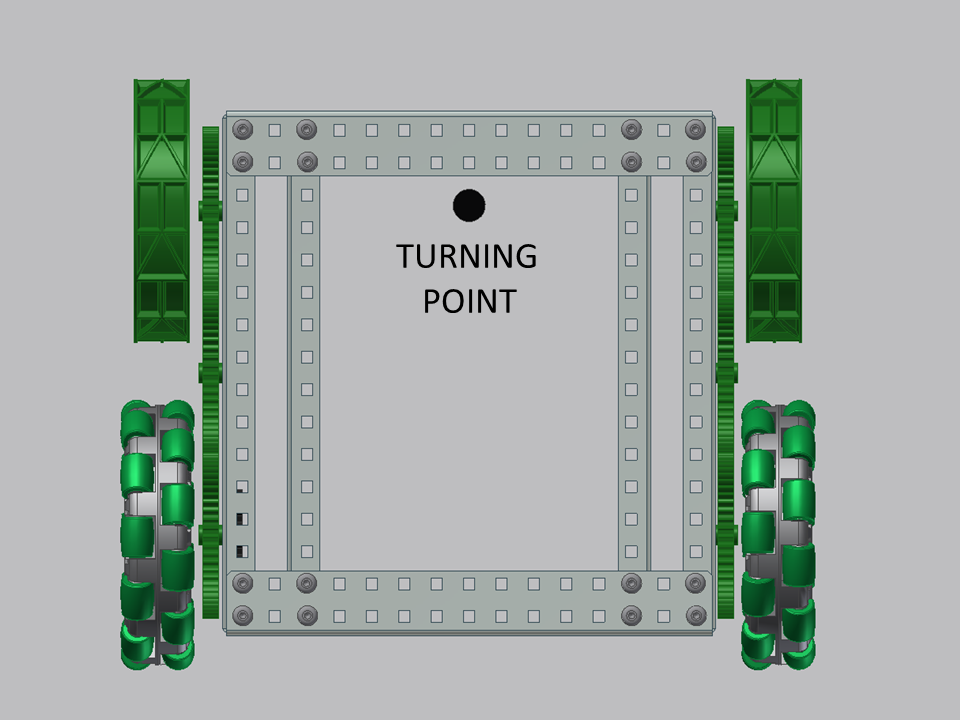
\includegraphics[height=265pt,width=\linewidth,keepaspectratio]{drivetrains/tankHalfOmniHalfTraction}
	\caption{A typical tank drive with half omni-wheels and half traction wheels}
	\label{fig:drivetrainTankHalfHalf}
\end{figure}

\subsection{Advantages}

\begin{itemize}
	\item Isn't prone to skiding like a tank drive with exclusivly omni-wheels
	\item Can be easily reconfigured to other kinds of drivetrain
\end{itemize}


\subsection{Disadvantages}

\begin{itemize}
	\item Turning point is on the edge of the robot, not the middle, reducing manuverability
\end{itemize}


\section{X-Drive}

<+descirption of drivetrain+>
\begin{figure}[h]
	\centering
	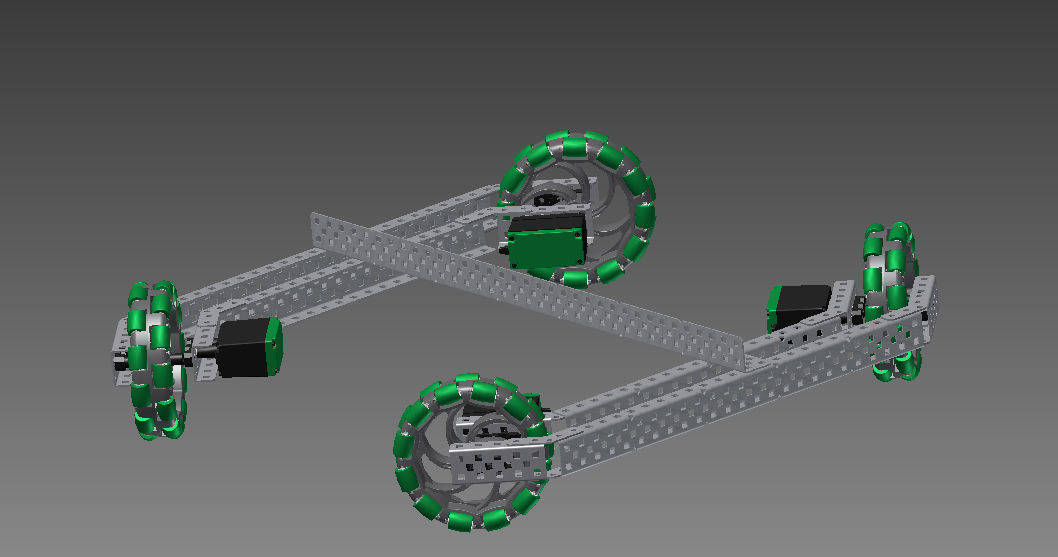
\includegraphics[height=265pt,width=\linewidth,keepaspectratio]{drivetrains/x}
	\caption{A typical X-Drive}
	\label{fig:drivetrainX}
\end{figure}

\subsection{Advantages}

\begin{itemize}
	\item Fast, moves at $\sqrt{2}$ times the speed of the wheel forward and sideways due to
	      both sets of wheels moving the robot.
	\item Holonomic

\end{itemize}


\subsection{Disadvantages}

\begin{itemize}
	\item Hard and unstable to build due to 45 \degree angles.
	\item Require four wheels, which is half the allowed motors
	      if we use a v5
\end{itemize}

\end{document}
